\section{Mesh Router}

\begin{frame}{Mesh Router}
%Danach geht der Vortrag auf den inneren Aufbau der Router Software
%(Firmware) ein. Es wird gezeigt, welche Aufgabe ein Router konkret
%zu erfüllen hat.

\begin{block}{
    \only<1-2>{Jeder Knoten ist wie ein großer Switch}
    \only<3-4>{Das Freifunk-Netz besteht aus}
}

\renewcommand{\arraystretch}{1.5}
\begin{tabular}{|c|c|c|c|c|c|c|} \hline
 \multicolumn{7}{|c|}{Bridge} \\ \hline
 \multirow{2}{*}{Managed} & \multicolumn{4}{c|}{\visible<2->{B.A.T.M.A.N}} & \multicolumn{2}{c|}{\multirow{2}{*}{Client-VLan}} \\ \cline{2-5}
 & \visible<3->{Ad-Hoc} & \visible<4->{VPN} & \multicolumn{2}{c|}{\visible<3->{Node-VLan}} & \multicolumn{2}{c|}{} \\ \hline
 \multicolumn{2}{|c|}{Wifi} & \visible<4->{WAN} & \visible<3->{LAN1} & \visible<3->{LAN2} & LAN3 & LAN4 \\ \hline
\end{tabular}

% TODO: Bridge/Managed/Clients grau machen, bei 3-4

\only<1-2>{
        \begin{itemize}
            \item Clients, die sich vor Ort per WLan verbinden
            \item Clients, die sich per Kabel verbinden
            \item<2> Das Freifunk-Netz
        \end{itemize}
}
\only<3-4>{
    \begin{itemize}
        \item Knoten, die sich über WLan verbinden
        \item Knoten, die sich über Kabel verbinden
        \item<4> Knoten, die über VPN verbunden werden
    \end{itemize}
}

\end{block}

\end{frame}


%\begin{frame}{Wifi - Ad-Hoc}
%    % TODO MAC Adressen ???
%\renewcommand{\arraystretch}{1.5}
%\begin{tabular}{|c|c|c|c|c|c|c|} \hline
% \multicolumn{7}{|c|}{Bridge :01} \\ \hline
% \multirow{2}{*}{Managed :01} & \multicolumn{4}{c|}{B.A.T.M.A.N :rr} & \multicolumn{2}{c|}{\multirow{2}{*}{Client-VLan :02}} \\ \cline{2-5}
% & Ad-Hoc :01 & VPN :rr & \multicolumn{2}{c|}{Node-VLan :02} & \multicolumn{2}{c|}{} \\ \hline
% \multicolumn{2}{|c|}{Wifi :01} & WAN :02 & LAN1 :02 & LAN2 :02 & LAN3 :02 & LAN4 :02 \\ \hline
%\end{tabular}
%
%\end{frame}

\begin{frame}{Anschlüsse}
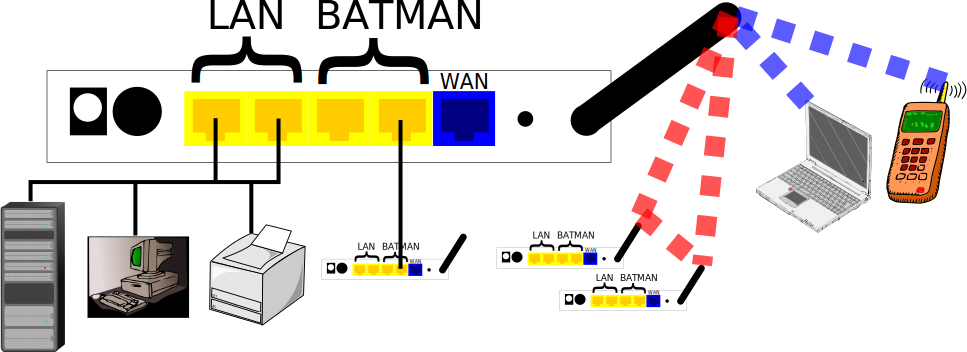
\includegraphics[width=0.75\textwidth]{img/svg/anschluesse.pdf}

An die Client Ports können beliebige Geräte an das Netz angeschlossen werden. Es ist auch mit einem Infrastructure Funknetz verbunden. Die Batman Ports, sowie das AdHoc Netz dienen zur Kommunikation zwischen den Routern. Der LAN-Port kann an ein bestehendes LAN angeschlossen werden und baut darüber einen Tunnel auf.
\end{frame}
